\documentclass[a4paper,12pt]{article}
\usepackage[utf8]{inputenc}
\usepackage[T1]{fontenc}
\usepackage{lmodern}
\IfFileExists{norsk.ldf}{\usepackage[norsk]{babel}}{}
\usepackage[a4paper,margin=2.5cm]{geometry}
\usepackage{amsmath,amssymb}
\usepackage{graphicx}
\usepackage{float}
\usepackage{parskip}
\usepackage{microtype}
\usepackage[hidelinks]{hyperref}
\renewcommand{\figurename}{Figur}
\pagestyle{plain}
\newcommand{\enhet}[1]{\,\mathrm{#1}}
% Samme plassering av hovedoverskrift som i A4- og A6-malen.
\newcommand{\oppgave}[1]{%
    \setlength{\topskip}{15.4pt}%
    \section*{Oppgave #1}%
    \setlength{\topskip}{12pt}%
    \vspace{1.363pt}%
}
\begin{document}
\oppgave{1}
Datasekvensen og bittiden er gitt som:
\[
    [0,1,0,1,1,0,1,0,1,0],\qquad T_b=62\enhet{\mu s}
\]
Bitraten finnes ved å ta den inverse av bittiden:
\[
    R_b=\frac{1}{T_b}=\frac{1}{62\cdot10^{-6}}
       \approx16129.032\enhet{bit/s}
\]
Ved NRZ beholder signalet samme nivå gjennom hele bittiden. Det raskest skiftende mønsteret er vekslende nuller og enere. En hel periode består da av to bit, og periodelengden blir:
\[
    T=2T_b=2\cdot62\enhet{\mu s}=124\enhet{\mu s}
\]
Grunnfrekvensen til dette mønsteret er:
\[
    f=\frac{1}{2T_b}=\frac{R_b}{2}
      \approx8064.516\enhet{Hz}
\]
Den minste teoretiske båndbredden for binær basisbåndsoverføring følger også fra Nyquist-grensen:
\[
    R_b\leq2B
\]
Dermed blir minste nødvendige kanalbåndbredde:
\[
    B_{\min}=\frac{R_b}{2}
            =\frac{16129.032}{2}
            \approx8064.516\enhet{Hz}
\]
Svaret, med den ideelle Nyquist-modellen for minste båndbredde, er:
\[
    \boxed{B_{\min}\approx8.065\enhet{kHz}}
\]

En ideell rektangulær NRZ-puls har et spektrum som strekker seg til uendelig frekvens. Den første spektralnullen ligger ved:
\[
    f_{\mathrm{null},1}=\frac{1}{T_b}=R_b\approx16.129\enhet{kHz}
\]
Dette er båndbredden fra null frekvens til første spektralnull. Svaret over gjelder den \emph{minste teoretiske kanalbåndbredden}, med ideell pulsforming og sampling uten intersymbolinterferens.

\clearpage
\oppgave{2}
Telefonkanalen har båndbredde og signal-støyforhold:
\[
    B=3.1\enhet{kHz}=3100\enhet{Hz},
    \qquad \mathrm{SNR}_{\mathrm{dB}}=36\enhet{dB}
\]

\subsection*{a)}
Først omregnes signal-støyforholdet til et lineært effektforhold:
\[
    \frac{S}{N}=10^{36/10}\approx3981.072
\]
Den teoretiske kanalkapasiteten finnes fra Shannon--Hartleys formel:
\[
    C=B\log_2\!\left(1+\frac{S}{N}\right)
\]
Vi setter inn kanaldataene:
\[
    C=3100\log_2(1+3981.072)
      \approx37073.841\enhet{bps}
\]
Den teoretisk største dataraten er dermed:
\[
    \boxed{C\approx37.074\enhet{kbps}}
\]

For å finne antallet symboltilstander sammenliknes dette med Nyquists uttrykk for $M$ tilstander ved maksimal symbolrate:
\[
    C=2B\log_2(M)
\]
Antallet bit per symbol ved den teoretiske grensen blir:
\[
    \log_2(M)=\frac{C}{2B}
             =\frac{37073.841}{2\cdot3100}
             \approx5.980
\]
Det formelle antallet symboltilstander blir derfor:
\[
    M=\sqrt{1+10^{36/10}}\approx63.104
\]
Resultatet av sammenlikningen er:
\[
    \boxed{M_{\mathrm{teor}}\approx63.104}
\]
Dette er en teoretisk referanseverdi, siden antallet tilstander må være et heltall. Avrundet opp kreves 64 tilstander for minst denne mengden informasjon per symbol (overskrider den teoretiske grensen).

\newpage
\subsection*{b)}
Vi bruker oppgavens modell med maksimal symbolrate og et fast, helt antall bit per symbol. Maksimal symbolrate er:
\[
    R_s=2B=2\cdot3100=6200\enhet{symbol/s}
\]
For $k$ bit per symbol er dataraten:
\[
    R_b=R_s k=2Bk
\]
Vi må velge det største heltallet $k$ som ikke gir en datarate over Shannon-grensen:
\[
    k\leq\frac{C}{2B}\approx5.980
\]
Dermed blir antallet bit per symbol:
\[
    k=\left\lfloor\frac{C}{2B}\right\rfloor=5
\]
Dette tilsvarer følgende antall symboltilstander:
\[
    M=2^k=2^5=32
\]
Dataraten i denne modellen blir:
\[
    R_b=6200\cdot5=31000\enhet{bps}
\]
Svaret for heltallskravet ved maksimal symbolrate er:
\[
    \boxed{R_b=31\enhet{kbps},\qquad k=5,\qquad M=32}
\]
Som kontroll ville seks bit per symbol ved samme symbolrate gitt:
\[
    R_b=6200\cdot6=37200\enhet{bps}
       >37073.841\enhet{bps}
\]
Dette overskrider Shannon-grensen og kan derfor ikke regnes som feilfri overføring med de oppgitte kanaldataene.

\clearpage
\oppgave{3}
Den største tilgjengelige verdien av bitenergi relativt til støytetthet er:
\[
    \left(\frac{E_b}{N_0}\right)_{\mathrm{dB}}=-0.450\enhet{dB}
\]
Den lineære verdien blir:
\[
    X=\frac{E_b}{N_0}=10^{-0.45/10}\approx0.902
\]
Vi betegner båndbreddeeffektiviteten med:
\[
    Y=\frac{C}{B}
\]
Bitenergien og støyeffekten kan uttrykkes som:
\[
    E_b=\frac{S}{C},\qquad N=N_0B
\]
Dette gir sammenhengen mellom signal-støyforhold og bitenergi:
\[
    \frac{S}{N}=\frac{E_bC}{N_0B}=XY
\]
Ved Shannon-grensen gjelder:
\[
    Y=\log_2\!\left(1+\frac{S}{N}\right)
\]
Vi setter inn uttrykket for signal-støyforholdet:
\[
    Y=\log_2(1+0.902Y)
\]
Her står den ukjente på begge sider. Vi løser derfor numerisk for den positive løsningen. Samme ligning kan skrives som:
\[
    \frac{2^Y-1}{Y}=0.902,\qquad Y>0
\]
For eksempel kan dette beregnes i Matlab/Octave uten ekstra toolbox:
\begin{verbatim}
X = 10^(-0.45/10);
f = @(Y) (2.^Y - 1)./Y - X;
Y = fzero(f, [0.7 0.75]);
C = 3100*Y;
disp(["Y = C/B =", num2str(Y)]);
\end{verbatim}
Den positive løsningen og største båndbreddeeffektiviteten blir:
\[
    \boxed{Y_{\max}\approx0.728\enhet{bps/Hz}}
\]
Løsningen $Y=0$ i den opprinnelige ligningen beskriver ingen informasjonsoverføring og er ikke den kapasiteten vi søker.

\newpage
Informasjonshastigheten innenfor den oppgitte båndbredden finnes fra:
\[
    C=Y_{\max}B
\]
Med $B=3100\enhet{Hz}$ blir dette, beregnet før avrunding av $Y_{\max}$:
\[
    C=Y_{\max}\cdot3100\approx2256.831\enhet{bps}
\]
Den teoretisk største informasjonshastigheten er dermed:
\[
    \boxed{C\approx2.257\enhet{kbps}}
\]
Som kontroll settes båndbreddeeffektiviteten tilbake i Shannon-uttrykket:
\[
    \log_2(1+0.902\cdot0.728)\approx0.728
\]
Figuren viser sammenhengen som brukes til å finne den positive løsningen:
\begin{figure}[H]
    \centering
    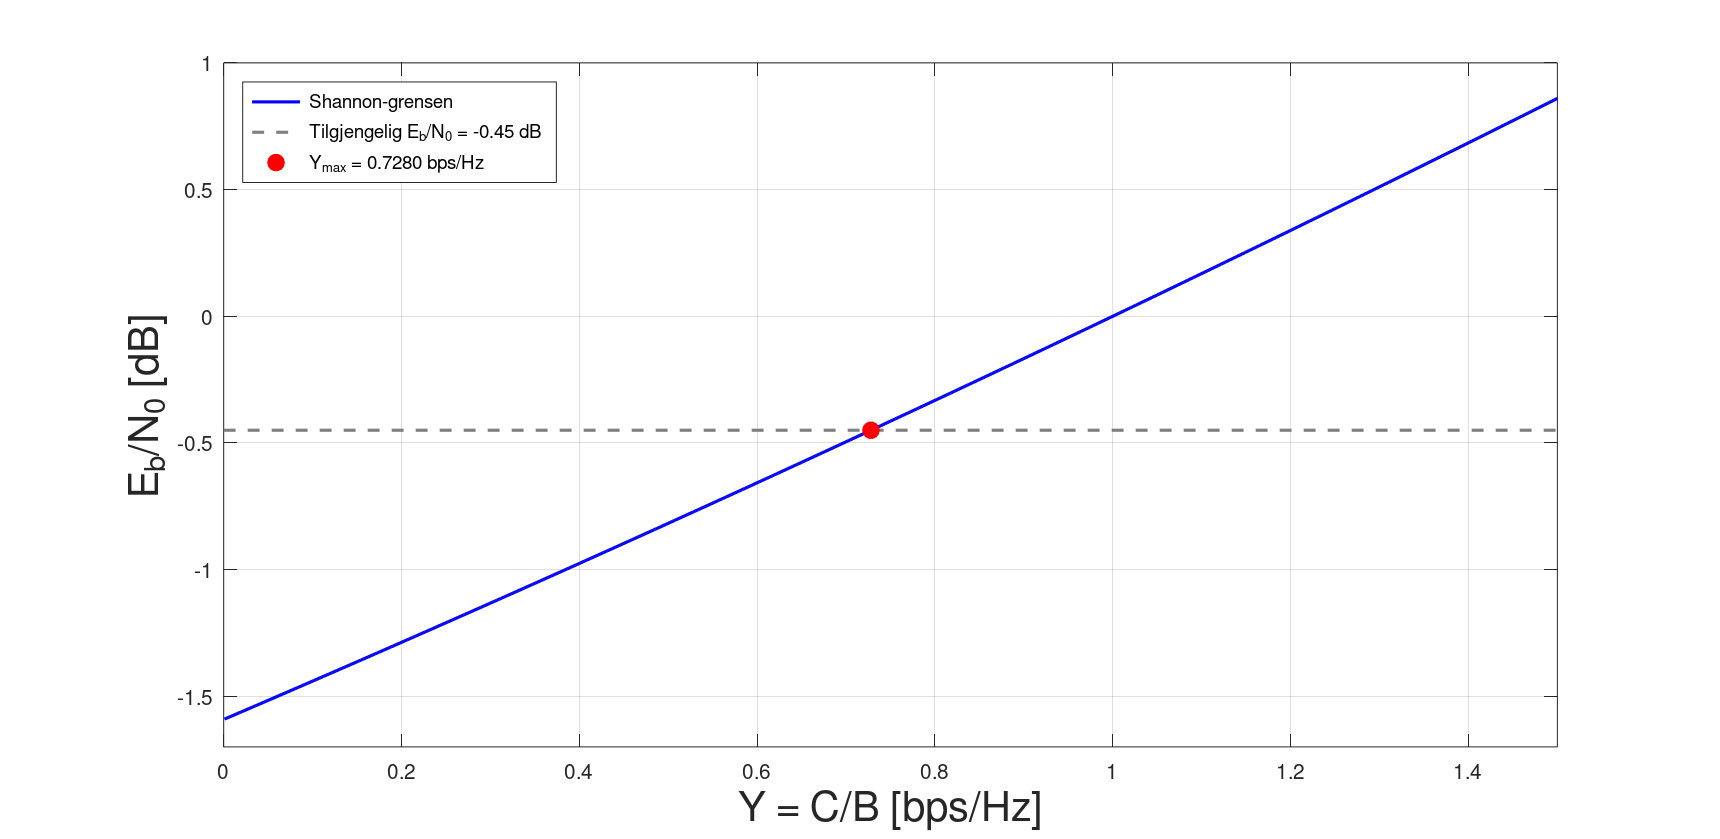
\includegraphics[width=\textwidth]{Media/grapf1.png}
    \caption{Shannon-grensen og tilgjengelig $E_b/N_0$ for undervannslenken.}
\end{figure}

\clearpage
\oppgave{4}
Den ønskede dataraten og signal-støyforholdet er:
\[
    R_b=56\enhet{kbps}=56000\enhet{bps},
    \qquad \mathrm{SNR}_{\mathrm{dB}}=-7\enhet{dB}
\]
Først omregnes signal-støyforholdet til lineær verdi:
\[
    \frac{S}{N}=10^{-7/10}\approx0.200
\]
Shannon--Hartleys formel gir den teoretiske kapasiteten:
\[
    C=B\log_2\!\left(1+\frac{S}{N}\right)
\]
For å kunne overføre datastrømmen må kapasiteten være minst lik dataraten:
\[
    B\log_2(1+10^{-7/10})\geq56000
\]
Vi løser med hensyn på båndbredden:
\[
    B\geq\frac{56000}{\log_2(1+10^{-7/10})}
\]
Dette gir minste teoretiske båndbredde ved det oppgitte signal-støyforholdet:
\[
    B_{\min}\approx213362.020\enhet{Hz}
\]
Svaret blir derfor:
\[
    \boxed{B_{\min}\approx213.362\enhet{kHz}}
\]

\clearpage
\oppgave{5}
Systemets båndbreddeeffektivitet er:
\[
    Y=\frac{C}{B}=3.75\enhet{bps/Hz}
\]
Ved Shannon-grensen er forholdet mellom effektiviteten og SNR gitt ved:
\[
    Y=\log_2\!\left(1+\frac{S}{N}\right)
\]
Vi opphøyer begge sider med grunntall 2:
\[
    2^Y=1+\frac{S}{N}
\]
Dermed er minste lineære signal-støyforhold:
\[
    \left(\frac{S}{N}\right)_{\min}=2^{3.75}-1
                                \approx12.454
\]
Dette omregnes til dB:
\[
    \mathrm{SNR}_{\min,\mathrm{dB}}
       =10\log_{10}(12.454)\approx10.953\enhet{dB}
\]
Minste nødvendige SNR er derfor:
\[
    \boxed{\mathrm{SNR}_{\min,\mathrm{dB}}\approx10.953\enhet{dB}}
\]
Sammenhengen med bitenergi relativt til støytetthet er:
\[
    \frac{S}{N}=\frac{E_b}{N_0}\frac{C}{B}
\]
Vi løser med hensyn på bitenergiforholdet og setter inn verdiene:
\[
    \frac{E_b}{N_0}=\frac{S/N}{C/B}
                  =\frac{12.454}{3.75}
                  \approx3.321
\]
Tilsvarende verdi i dB blir:
\[
    \left(\frac{E_b}{N_0}\right)_{\mathrm{dB}}
       =10\log_{10}(3.321)\approx5.213\enhet{dB}
\]
Vi har dermed:
\[
    \boxed{\frac{E_b}{N_0}\approx3.321,
    \qquad \left(\frac{E_b}{N_0}\right)_{\mathrm{dB}}\approx5.213\enhet{dB}}
\]

\clearpage
\oppgave{6}
Den binære basisbåndsoverføringen har kanalbåndbredde og roll-off-faktor:
\[
    B=35\enhet{kHz}=35000\enhet{Hz},\qquad\alpha=0.65
\]
Et Raised Cosine-filter har følgende sammenheng mellom den ensidige basisbåndbredden og symbolraten:
\[
    B=\frac{1+\alpha}{2}R_s
\]
Ved binær overføring er det en bit per symbol, slik at:
\[
    R_b=R_s
\]
Vi kan derfor skrive båndbreddekravet som:
\[
    B=\frac{1+\alpha}{2}R_b
\]
Vi løser med hensyn på bitraten:
\[
    R_b=\frac{2B}{1+\alpha}
\]
De oppgitte verdiene settes inn:
\[
    R_b=\frac{2\cdot35000}{1+0.65}
       =\frac{70000}{1.65}
       \approx42424.242\enhet{bps}
\]
Den forventede kapasiteten ut fra båndbredde og pulsforming er dermed:
\[
    \boxed{R_b\approx42.424\enhet{kbps}}
\]

\clearpage
\oppgave{7}
Den opprinnelige bitraten og de to roll-off-faktorene er:
\[
    R_{b,1}=6400\enhet{bps},\qquad
    \alpha_1=0.55,\qquad\alpha_2=0.15
\]
Vi antar at kanalbåndbredden beholdes. Båndbredden for den opprinnelige binære overføringen er:
\[
    B=\frac{1+\alpha_1}{2}R_{b,1}
\]
Vi setter inn verdiene:
\[
    B=\frac{1+0.55}{2}\cdot6400=4960\enhet{Hz}
\]
Når roll-off-faktoren reduseres, kan bitraten økes innenfor samme båndbredde:
\[
    R_{b,2}=\frac{2B}{1+\alpha_2}
\]
Den nye bitraten blir:
\[
    R_{b,2}=\frac{2\cdot4960}{1+0.15}
           \approx8626.087\enhet{bps}
\]
Vi kunne også funnet dette direkte fra forholdet mellom roll-off-faktorene:
\[
    R_{b,2}=R_{b,1}\frac{1+\alpha_1}{1+\alpha_2}
           =6400\frac{1.55}{1.15}
           \approx8626.087\enhet{bps}
\]
Økningen i bitrate er:
\[
    \Delta R_b=8626.087-6400\approx2226.087\enhet{bps}
\]
Den prosentvise økningen blir:
\[
    \frac{R_{b,2}-R_{b,1}}{R_{b,1}}\cdot100\%
       =\frac{2226.087}{6400}\cdot100\%
       \approx34.783\%
\]
Informasjonen kan dermed sendes med:
\[
    \boxed{R_{b,2}\approx8.626\enhet{kbps},
    \quad\text{en økning på }34.783\%}
\]
En lavere roll-off-faktor gir mindre overskuddsbåndbredde, men stiller samtidig strengere krav til pulsforming og tidsstyring i mottakeren (mindre robust mot jitter).

\clearpage
\oppgave{8}
Vi tolker bipolar NRZ i oppgaven som antipodal, binær signalering med to motsatte spenningsnivåer, altså $-A$ og $+A$. Vi antar like sannsynlige bit, additiv hvit Gauss-støy og optimal deteksjon uten intersymbolinterferens. Bitfeilsannsynligheten er da:
\[
    \mathrm{BER}=P_b=Q\!\left(\sqrt{\frac{2E_b}{N_0}}\right)
\]
$Q$-funksjonen gir sannsynligheten for at en standard normalfordelt variabel er større enn argumentet.

\subsection*{a)}
Kravet til bitfeilsannsynlighet er:
\[
    Q\!\left(\sqrt{\frac{2E_b}{N_0}}\right)\leq10^{-6}
\]
Siden $Q(x)$ er avtakende, finner vi minste nødvendige bitenergiforhold ved å sette BER lik grenseverdien:
\[
    \sqrt{\frac{2E_b}{N_0}}=Q^{-1}(10^{-6})
\]
Verdien av $Q^{-1}(10^{-6})$ må finnes fra en normalfordelingstabell eller en numerisk funksjon. Den inverse funksjonen finner argumentet som gir den ønskede halesannsynligheten, og er ikke det samme som $1/Q$.

En beregning uten ekstra Matlab/Octave-toolbox bruker sammenhengen med den komplementære feilfunksjonen og dens inverse:
\begin{align*}
    Q(x)&=\frac{1}{2}\operatorname{erfc}\!\left(\frac{x}{\sqrt{2}}\right)\\
    Q^{-1}(p)&=\sqrt{2}\operatorname{erfc}^{-1}(2p)
\end{align*}
For det oppgitte BER-kravet blir beregningen:
\[
    Q^{-1}(10^{-6})=\sqrt{2}\operatorname{erfc}^{-1}(2\cdot10^{-6})
                  \approx4.753
\]
Den samme tallverdien beregnes i Matlab/Octave med:
\begin{verbatim}
x = sqrt(2)*erfcinv(2*1e-6);
\end{verbatim}
Vi kvadrerer og deler på 2 for å finne den lineære verdien:
\[
    \left(\frac{E_b}{N_0}\right)_{\min}
       =\frac{(4.753)^2}{2}\approx11.298
\]
Dette omregnes til dB:
\[
    \left(\frac{E_b}{N_0}\right)_{\min,\mathrm{dB}}
       =10\log_{10}(11.298)\approx10.530\enhet{dB}
\]
Minste verdi som oppfyller BER-kravet er derfor:
\[
    \boxed{\left(\frac{E_b}{N_0}\right)_{\min}\approx11.298,
    \quad\left(\frac{E_b}{N_0}\right)_{\min,\mathrm{dB}}\approx10.530\enhet{dB}}
\]

\newpage
\subsection*{b)}
Det oppgitte bitenergiforholdet er:
\[
    \left(\frac{E_b}{N_0}\right)_{\mathrm{dB}}=11\enhet{dB}
\]
Først omregnes det til lineær verdi:
\[
    \frac{E_b}{N_0}=10^{11/10}\approx12.589
\]
Dette settes inn i BER-uttrykket for antipodal NRZ:
\[
    P_b=Q\!\left(\sqrt{2\cdot12.589}\right)
\]
Argumentet til $Q$-funksjonen blir:
\[
    x=\sqrt{25.178}\approx5.018
\]
Ved å bruke den komplementære feilfunksjonen får vi:
\[
    P_b=\frac{1}{2}\operatorname{erfc}\!\left(    \frac{5.018}{\sqrt{2}}\right)
       \approx2.613\cdot10^{-7}
\]
Dette kan beregnes direkte i Matlab/Octave med:
\begin{verbatim}
Y = 10^(11/10);
BER = 0.5*erfc(sqrt(Y));
\end{verbatim}
Den forventede bitfeilsannsynligheten er dermed:
\[
    \boxed{\mathrm{BER}\approx2.613\cdot10^{-7}}
\]
Dette er lavere enn $10^{-6}$, i samsvar med at $11\enhet{dB}$ er høyere enn den nødvendige minsteverdien fra a).

\clearpage
\oppgave{9}
Systemets bitrate og bitenergiforhold er:
\[
    R_b=48\enhet{kbps}=48000\enhet{bps},\qquad
    \left(\frac{E_b}{N_0}\right)_{\mathrm{dB}}=7.5\enhet{dB}
\]
Vi bruker ideell Nyquist-båndbredde for binær overføring i basisbånd.

BER-uttrykkene forutsetter like sannsynlige bit, additiv hvit Gauss-støy og optimal deteksjon uten intersymbolinterferens.

\subsection*{a)}
Sammenhengen mellom signal-støyforhold og bitenergiforhold er:
\[
    \frac{S}{N}=\frac{E_b}{N_0}\frac{R_b}{B}
\]
Ved minste båndbredde for binær basisbåndsoverføring gjelder:
\[
    B_{\min}=\frac{R_b}{2},\qquad\frac{R_b}{B_{\min}}=2
\]
I dB kan sammenhengen skrives som:
\[
    \left(\frac{S}{N}\right)_{\mathrm{dB}}
       =\left(\frac{E_b}{N_0}\right)_{\mathrm{dB}}
        +10\log_{10}\!\left(\frac{R_b}{B}\right)
\]
Med minste båndbredde får vi:
\[
    \left(\frac{S}{N}\right)_{\mathrm{dB}}
       =7.5+10\log_{10}(2)
       =7.5+3.010\approx10.510\enhet{dB}
\]
Signal-støyforholdet er derfor:
\[
    \boxed{\left(\frac{S}{N}\right)_{\mathrm{dB}}\approx10.510\enhet{dB}}
\]

\subsection*{b)}
Den minste teoretiske båndbredden finnes fra Nyquist-grensen:
\[
    B_{\min}=\frac{R_b}{2}=\frac{48000}{2}=24000\enhet{Hz}
\]
Svaret blir:
\[
    \boxed{B_{\min}=24\enhet{kHz}}
\]

\newpage
\subsection*{c)}
For unipolar NRZ med nivåene $0$ og $A$ brukes gjennomsnittlig energi per bit. Bitfeilsannsynligheten ved optimal terskel er:
\[
    P_{b,\mathrm{uni}}=Q\!\left(\sqrt{\frac{E_b}{N_0}}\right)
\]
Det oppgitte bitenergiforholdet omregnes til lineær verdi:
\[
    \frac{E_b}{N_0}=10^{7.5/10}\approx5.623
\]
Vi setter inn verdien og beregner argumentet til $Q$-funksjonen:
\[
    P_{b,\mathrm{uni}}=Q(\sqrt{5.623})=Q(2.371)
\]
Den numeriske verdien kan beregnes med feilfunksjonen:
\[
    P_{b,\mathrm{uni}}=\frac{1}{2}\operatorname{erfc}\!\left(
        \frac{2.371}{\sqrt{2}}\right)
        \approx8.861\cdot10^{-3}
\]
Bitfeilsannsynligheten for unipolar NRZ er dermed:
\[
    \boxed{\mathrm{BER}_{\mathrm{uni}}\approx8.861\cdot10^{-3}
    \approx0.886\%}
\]
Hvis feilhyppigheten uttrykkes som forventet antall bitfeil per sekund, blir den:
\[
    R_bP_{b,\mathrm{uni}}
       =48000\cdot8.861\cdot10^{-3}
       \approx425.330\enhet{beps}
\]

\subsection*{d)}
For bipolar NRZ med nivåene $-A$ og $+A$, brukes:
\[
    P_{b,\mathrm{bi}}=Q\!\left(\sqrt{\frac{2E_b}{N_0}}\right)
\]
Vi setter inn det samme bitenergiforholdet som i c):
\[
    P_{b,\mathrm{bi}}=Q(\sqrt{2\cdot5.623})
                     =Q(3.354)
\]
Den numeriske bitfeilsannsynligheten blir:
\[
    \boxed{\mathrm{BER}_{\mathrm{bi}}\approx3.988\cdot10^{-4}
    \approx0.040\%}
\]
Dette tilsvarer følgende forventede antall bitfeil per sekund:
\[
    48000\cdot3.988\cdot10^{-4}
                        \approx19.142\enhet{beps}
\]
Vi får lavere BER ved samme gjennomsnittlige bitenergi, fordi de to signaltilstandene ligger lenger fra hverandre.

\end{document}
